\section{Przykłady działania aplikacji}
Po uruchomieniu aplikacji celem \textbf{run\_local} oczom użytkownika ukaże się
okno klienta oraz terminal wypełniony informacjami diagnostycznymi.\\

Przykładowa prezentacja:
\begin{figure}[H]
    \centering
    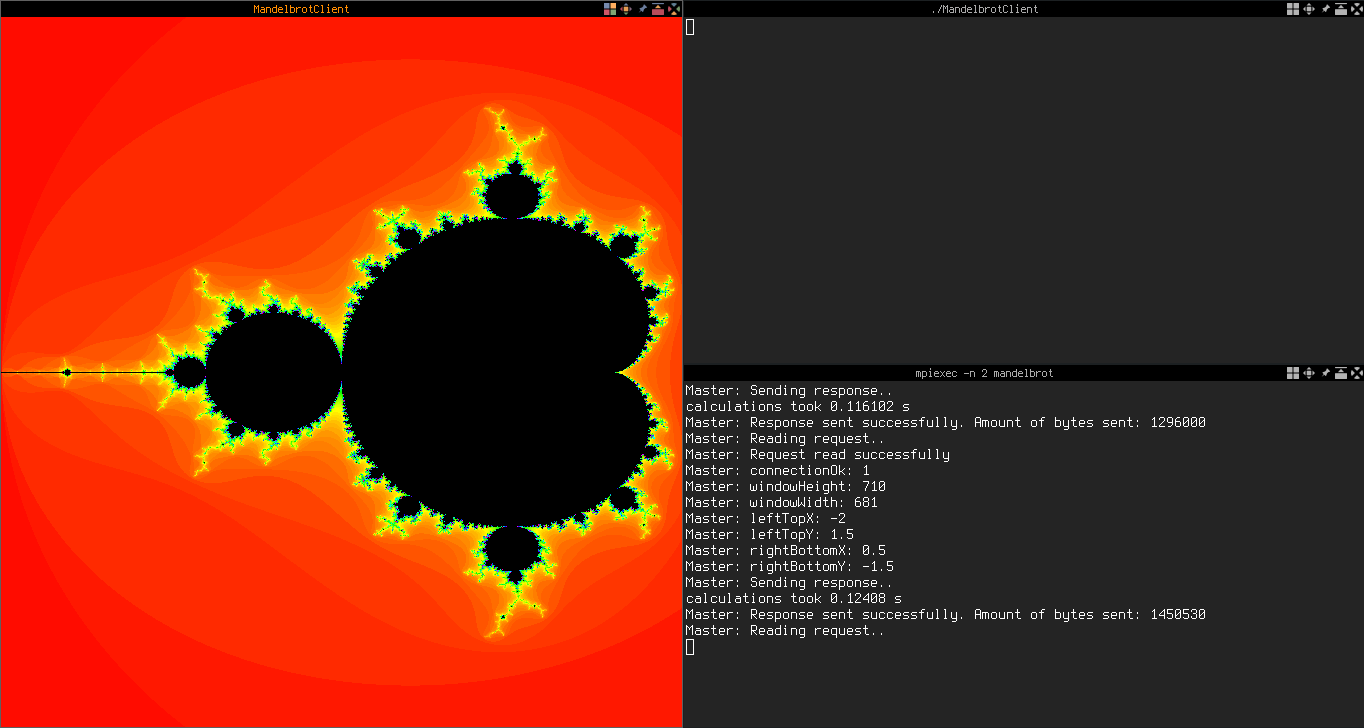
\includegraphics[width = \textwidth]{img/ex1.png}
\end{figure}

\begin{figure}[H]
    \centering
    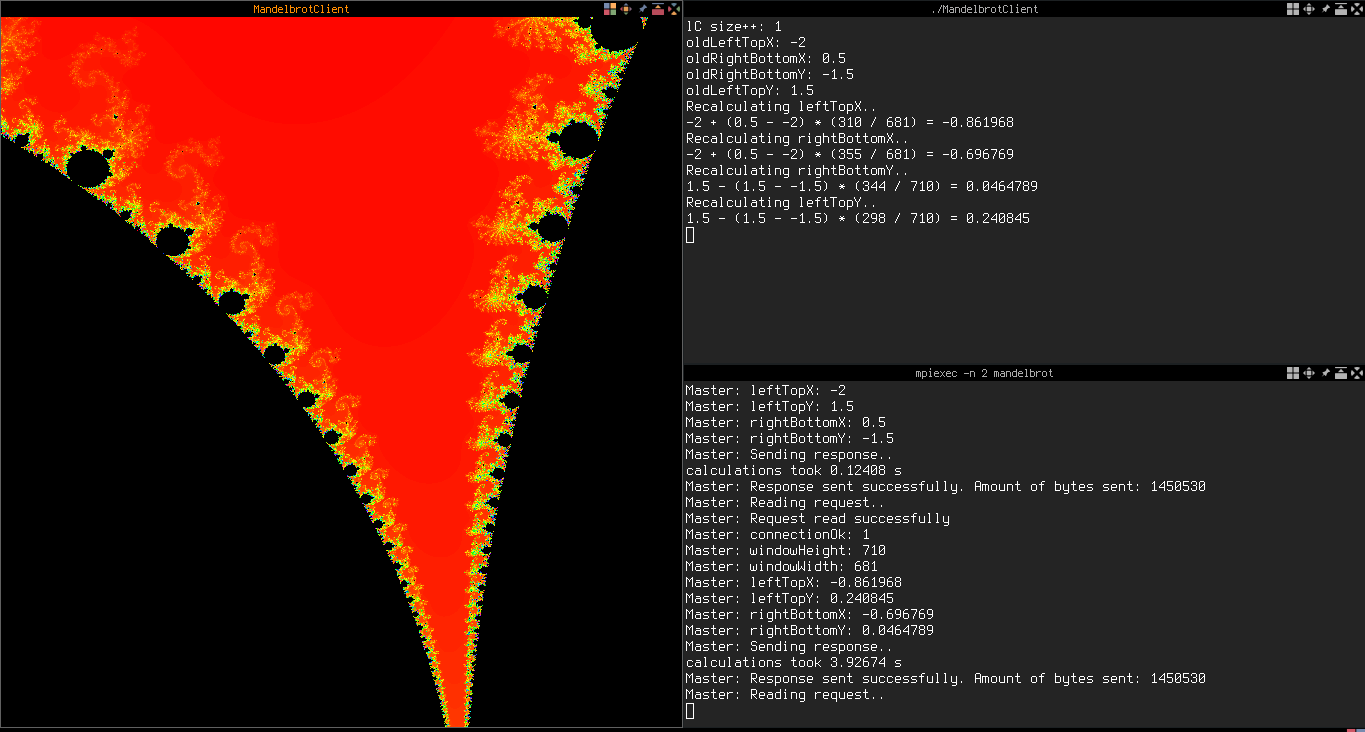
\includegraphics[width = \textwidth]{img/ex2.png}
\end{figure}

Jak można zaobserwować na poniższym obrazie aplikacja pozwala uzyskać znaczne przybliżenie na elementy zbioru.
\begin{figure}[H]
    \centering
    
\includegraphics[width = 0.7\textwidth]{img/ex3.png}
\end{figure}